\chapter{Evaluation of API Overwriting in Popular Websites}
\label{sec.evaluation}

One of the goals of this thesis is to evaluate the prevalence of browser \acs{api} manipulation. Analyzing web pages at a large scale requires automating the process of visiting these pages and collecting the results produced by the browser extension described in \autoref{sec.browserExtension}. \autoref{sec.automation-architecture} of this chapter provides an overview of the infrastructure created to handle the automation of the aforementioned processes and \autoref{sec.findings} presents the results of the collected data and highlights interesting findings. Furthermore, it will give insight into what kind of \acsp{api} are overwritten and showcase different use-cases for browser API manipulation.



\section{Automated Analysis Infrastructure}
\label{sec.automation-architecture}

To analyze the prevalence of browser \acs{api} manipulation, the extension is used in addition to an automated system that controls a browser and visits a list of websites while gathering relevant information such as which \acsp{api} have been overwritten and where the modification originated from. Figure \ref{fig.automation} shows the four core components of the automation infrastructure: the automation script, browser, browser extension and data collection script. The automation script is written in Python and makes use of the Playwright Python library, which allows automating browsers based on Chromium, Firefox and WebKit with a single \acs{api} \cite{PlaywrightPython}. It starts the browser – in this case Chromium version \icode{101.0.4951.15} – and instructs it to load the extension using the \icode{--load-extension=<path>} argument. The browser is then automated to open a new tab for each domain and close it again after the page has finished loading and an additional delay of five seconds has passed, which ensures that the page has reached its final state and gives the extension enough time to analyze the page and send the resulting data to the collection script. The result of each page is encoded as \acs{json} and sent from the browser extension to another script via an \acs{http} request. The data collection script implements a simple \acs{rest}~\acs{api} that receives the \acs{json} payload and stores it for further analysis.

\begin{figure}[H]
    \centering
    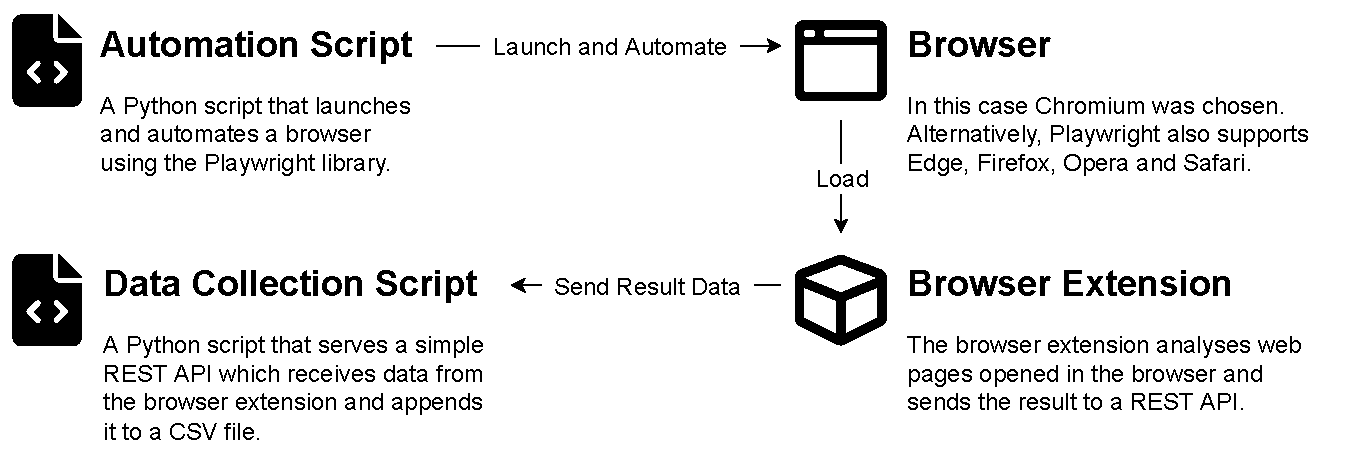
\includegraphics[width=16cm]{img/automation.pdf}
    \caption{Overview of the automation infrastructure}
    \label{fig.automation}
\end{figure}

\filbreak{}

The evaluation presented in this chapter analyzes the \num[round-precision=0]{16000} most popular domains acquired from the Tranco list \cite{Tranco} for the 3rd of May, 2022. The Tranco list was chosen due to its focus on providing a list suitable for research. It has the benefit of being available free of charge and allows reproducible results due to the permanent availability of historical lists. Since the list bases its domain ranking on a combination of data from different datasets such as Alexa, Cisco Umbrella and Majestic, it provides a more accurate representation of real-world popularity and better resistance against manipulation compared to its sources. \cite{Tranco}

Domains are processed in parallel, with limits on how many pages are processed at the same time and how long each page is allowed to load for. After testing different values for these limits, the ideal configuration in terms of performance and reliability for the machine that the automation was tested on seem to be a maximum of twice as much tabs open at the same time as the amount of available \acs{cpu} cores, and a timeout of $75$ to $90$ seconds. The timeouts are necessary in order to prevent pages with long loadings times from accumulating, which would slow down the script and potentially cause it to get stuck waiting indefinitely for unresponsive pages.



\section{Results of the Evaluation}
\label{sec.findings}

This section presents the results of the evaluation of API overwriting in popular websites. The first paragraph discusses the success rate and explains why certain domains included in the Tranco list did not produce a result. The following paragraphs discuss the most commonly overwritten \acsp{api} and present use-cases for these modifications.

Out of the \num[round-precision=0]{16000} domains that where processed, \SI[round-precision=0]{17.91}{\percent} failed to load or did not produce a result. This has various reasons, with the most common one being that not all domains included in the Tranco list host web pages. Domains such as \icode{akamaiedge.net} are used for \acp{cdn}, which act as proxies that cache and deliver resources such as images, audio, videos or scripts. Other domains like \icode{doubleclick.net} serve advertisements, and domains such as \icode{adobe.io} offer \acs{http}~\acsp{api}. Additionally, some domains only redirect to other domains, like \icode{youtu.be} and \icode{bit.ly}. The Tranco list also includes domains that only serve web content on subdomains, but does not include any subdomains (e.g. \icode{sub.example.com}) in the list, only the \ac{esld} (e.g. \icode{example.com}). One example of such a domain is \icode{wixsite.com}, which only serves web content on subdomains in the form of \icode{example.wixsite.com} that can be registered by users.

A visualization of the success rate and the prevalence of certain properties, such as how many sites included external scripts that modified \browserAPIs{}, can be seen in \autoref{fig.evaluation-overview}. The following sections will address these properties in more detail.

\begin{figure}[H]
    \centering
    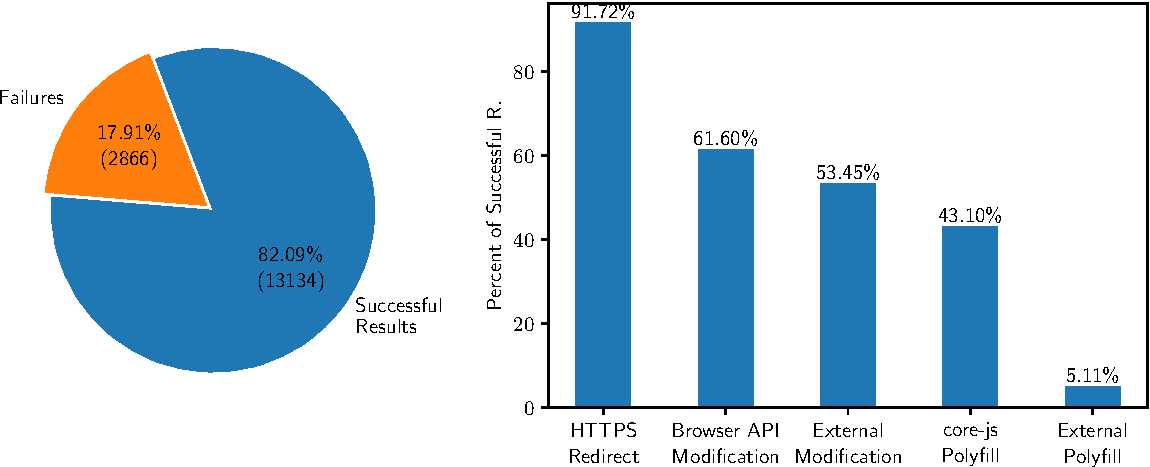
\includegraphics[width=16cm]{img/evaluation-overview.pdf}
    \caption{Failure rate (left) and prevalence of certain properties (right)}
    \label{fig.evaluation-overview}
\end{figure}

The results show that it is common practice to overwrite \acsp{api}, even when an up-to-date browser is used. In total, \SI[round-precision=0]{61.60}{\percent} of the successfully processed domains modified at least one browser \ac{api}. The ten most commonly overwritten \acs{api} methods and the percentage of domains that overwrote them can be seen in \autoref{tab.apisTop10}, while a more extensive list is available in appendix \ref{tab.apis}. With approximately \SI[round-precision=0]{44.12}{\percent} and \SI[round-precision=0]{40.79}{\percent} of affected domains respectively, the two most commonly modified \acsp{api} are \icode{history.pushState()} and \icode{history.replaceState()}. These functions can be used to add items to the browser session history or modify existing items in the history, as long as the URLs of the history items are part of the same origin as the current location \cite{MozPushState, MozReplaceState}. JavaScript libraries such as Google Tag Manager, Meta (formerly known as Facebook) Pixel Tracker and the Tiktok Pixel Tracker overwrite the aforementioned functions to track which pages a user visits and how they interact with the web application. Some domains even include multiple libraries that all overwrite the same function. In the case of \icode{wordpress.com}, the \icode{pushState} function is overwritten by the following five external libraries: Google Tag Manager, Meta Pixel Tracker, Microsoft Clarity (user session recording), Olark (live chat) and Outbrain (advertisement and recommendations). These overwrites each add an additional wrapper around the native browser \acs{api}, but – at least in this case – do not seem to interfere with each other.

\begin{table}[h]
    \parbox{\linewidth}{
    \centering
    \begin{tabular}{|r|l|}
    \hline
    Percentage & API Method \\
    \hline
    44.12 & \minline{history.pushState}\\
    40.79 & \minline{history.replaceState}\\
    13.64 & \minline{fetch}\\
    11.88 & \minline{setTimeout}\\
     8.22 & \minline{setInterval}\\
     6.96 & \minline{Math.sinh}\\
     6.76 & \minline{parseInt}\\
     6.79 & \minline{requestAnimationFrame}\\
     6.62 & \minline{clearTimeout}\\
     6.57 & \minline{XMLHttpRequest}\\
    \hline
    \end{tabular}
    }
    \caption{Top 10 most commonly modified APIs and percentage of affected domains}
    \label{tab.apisTop10}
\end{table}

\filbreak{}

The results also make it clear that the usage of polyfill libraries is very common. The polyfill library core-js is used by \SI[round-precision=0]{43.10}{\percent} of domains and more than \SI[round-precision=0]{5.11}{\percent} of web applications included polyfills from third-party domains. \autoref{tab.polyfill-domains} shows the 10 most popular services for external polyfills, with the most common one being \icode{polyfill.io}.

The low amount of externally included polyfill libraries seems to indicate that the libraries are usually hosted on first-party domains or subdomains, which is a good way to reduce the attack surface since there is less trust being placed on third-parties. It is surprising, however, to see government pages such as \icode{www.texas.gov} and even financial platforms such as \icode{www.blockchain.com} include external scripts from third-parties such as \icode{polyfill.io}.

\begin{table}[h]
    \centering
    \begin{tabular}{|r|l|}
    \hline
    Percent & Domain \\
    \hline
    2.84 & polyfill.io\\
    0.30 & gannettdigital.com\\
    0.29 & cloudflare.com\\
    0.24 & alicdn.com\\
    0.13 & jsdelivr.net\\
    0.13 & cloudfront.net\\
    0.12 & jwpcdn.com\\
    0.09 & squarespace.com\\
    0.06 & unpkg.com\\
    0.06 & wp.com\\
    \hline
    \end{tabular}
    \caption{Top 10 most common third-party domains delivering polyfill libraries and percentage of successfully analyzed domains using them}
    \label{tab.polyfill-domains}
\end{table}

The list of modified functions only includes a single instace where an existing cryptography \acsp{api} was overwritten, which will be investigated in \autoref{sec.investigationOfObfuscatedFunc}. In this case, however, there was no evidence for the threats as described in \autoref{sec.threats.crypto}. There are two cases in which websites added new functions to the crypto \acs{api}. These new functions are not used as replacements for existing functionality, but instead offer utilities for converting between different encodings (such as bytes, hexadecimal or base64) and an implementation of the cryptographically insecure md5 hash algorithm.

A browser \acs{api} that is commonly overwritten, is the fetch \acs{api}. With \SI[round-precision=0]{13.64}{\percent} of the analyzed domains modifying \icode{fetch}, it is the third most commonly overwritten browser \acs{api}. Investigations of some of these cases has revealed that this is done to customize its behavior and monitor web applications. This is also done by the “sentry” library for example, which overwrites \icode{fetch} and \icode{console} methods to monitor and collect data about the behavior of web applications. As listed in \autoref{tab.modifying-domains}, sentry modifies browser \acsp{api} in \SI[round-precision=2]{0.49}{\percent} of the scanned domains.

Since the automation script opens \acp{url} with the insecure \acs{http} by default, it was also measured how many web servers automatically redirect to \acs{https}, as instructed by the browser via the \icode{Upgrade-Insecure-Requests} header which all browsers are required to send along with insecure requests \cite{UpgradeInsecureRequests}. Out of the successfully processed domains, \SI[round-precision=0]{91.72}{\percent} redirected to \acs{https}. The domains that do not redirect to \acs{https} include government websites such as \icode{www.chinatax.gov.cn}, which also does not use a trusted certificate authority and therefore browsers show a security warning when manually specifying that \acs{https} should be used.

\section{Case Study of an Obfuscated API Overwrite}
\label{sec.investigationOfObfuscatedFunc}

This section will investigate an overwrite of the \icode{crypto.getRandomValues()} \ac{api} by an obfuscated script. The overwrite was detected during the automated evaluation and identified on the real estate web application \icode{zillow.com}.

The function that \icode{crypto.getRandomValues()} was replaced with is depicted in \autoref{lst.obfuscatedFunc}. Due to the obfuscation technique, it is not apparent how this function behaves. Furthermore, the code references variables such as \icode{c} and \icode{t} that are defined outside of the function.

\begin{lstlisting}[language=JavaScript,breaklines=true,breakatwhitespace=false,label={lst.obfuscatedFunc},caption={Obfuscated function}]
function n(){try{var i=3===++c,o=this&&Object.getPrototypeOf(this)===n.prototype||!1,u={P:o?null:this,L:Array.prototype.slice.call(arguments),$:null},a=!1;if(i)lu(Error(),E);else if(r)try{r(u)}catch(t){a=!0}if(o?u.P=u.$=Le(t,$e(u.L)):u.$=t.apply(u.P,u.L),!i&&!a&&e)try{e(u)}catch(t){}return u.$}finally{c--}}
\end{lstlisting}

In order to attempt to reverse engineer the function, the script responsible for the overwrite was examined. The URL of the script is \icode{https://www.zillow.com/HYx10rg3/init.js}, which means that it does not originate from a third-party domain. However, it is possible that this code was included by a third-party JavaScript library. This seems to be the case, as the file contains a header with the following comment:\\
\icode{// @license Copyright (C) 2014-2022 PerimeterX, Inc (www.perimeterx.com).}\\
\icode{Content of this file can not be copied and/or distributed.} % haha, we will see about that lol

The relevant content of the file is listed in \autoref{lst.obfuscatedScript}. Line breaks and indentation were added to improve the readablility. While the code is still difficult to understand, we can see that the function \icode{n} from \autoref{lst.obfuscatedFunc} is contained in the lines 5 to 32 of \autoref{lst.obfuscatedScript}. Some of the previously unknown variables are defined in lines 2 to 4 and received as arguments in line 1. The function in line 33 to 48 creates properties on the object \icode{t} and overwrites its \icode{toString()} method, which suggests that \icode{t} is the \browserAPI{} being overwritten and this is an attempt at hiding the true string value, which would reveal that the \ac{api} was overwritten.

\begin{lstlisting}[language=JavaScript,breaklines=true,breakatwhitespace=true,label={lst.obfuscatedScript},caption={Content of obfuscated script}]
function qe(t, n) {
    var r = n._ || null
        , e = n.U || null
        , c = 0
        , i = function n() {
        try {
            var i = 3 === ++c
                , o = this && Object.getPrototypeOf(this) === n.prototype || !1
                , u = {
                P: o ? null : this,
                L: Array.prototype.slice.call(arguments),
                $: null
            }
                , a = !1;
            if (i)
                lu(Error(), E);
            else if (r)
                try {
                    r(u)
                } catch (t) {
                    a = !0
                }
            if (o ? u.P = u.$ = Le(t, $e(u.L)) : u.$ = t.apply(u.P, u.L),
            !i && !a && e)
                try {
                    e(u)
                } catch (t) {}
            return u.$
        } finally {
            c--
        }
    };
    return function(t, n) {
        try {
            Object.defineProperty(t, "name", {
                value: n.name
            })
        } catch (t) {}
        try {
            Object.defineProperty(t, "length", {
                value: n.length
            })
        } catch (t) {}
        "function" == typeof n.toString && (t.toString = function() {
            return n.toString()
        }
        )
    }(i, t),
    i
}
\end{lstlisting}

Using the additional context gained through the surrounding code, an attempt was made to reverse engineer the function \icode{n} in line 5 of \autoref{lst.obfuscatedFunc}. First, a break-point was set at the beginning of the function through the Chromium developer tools. Next, the function was called with \icode{crypto.getRandomValues(new Uint32Array(42));} and then stepped through, in order to assess its behavior. During each step, the values of the variables were noted down to get a better understanding of their use. The final reverse engineered function is shown in \autoref{lst.reverseEngineeredFunc}. Variables have been renamed to reflect their purpose and the code has been restructured in order to improve readability.

While some functions and variables referenced in the code of \autoref{lst.reverseEngineeredFunc} are still not entirely s, the function previously called \icode{n} seems to be designed to act as a wrapper around the native \ac{api}. The wrapper function allows adding hooks that are called before and after the native \ac{api}. In this case, \icode{preHook} references another function and \icode{postHook} is undefined. The \icode{preHook} function, which is defined in another section of the code that is not included here, checks if the requested type for the random values is \icode{Uint8Array} and has the length \icode{16}. Calling \icode{rypto.getRandomValues(new Uint8Array(16));} results in the hook executing further functions, however, those do not manipulate the returned value.

\filbreak{}

Since the wrapper function calls the native \icode{crypto.getRandomValues()} API and returns its result unmodified, this does not seem to be a malicious \browserAPI{} overwrite. However, the complete behavior of the function could not be reverse engineered due to the high complexity and obfuscation of the code.

While this case study could not identify malicious behavior, it demonstrates the complexity involved in reverse engineering and classifying whether manipulations are malicious.

\par{}

\begin{lstlisting}[language=JavaScript,breaklines=true,breakatwhitespace=false,label={lst.reverseEngineeredFunc},caption={Attempt at reverse engineering the obfuscated function}]
/* Variables defined outside */
// Reference to original function
var nativeGetRandomValues = crypto.getRandomValues;

var preHook = wrapper.preHook || null
var postHook = wrapper.postHook || null

// Counter of failed attempts
var attempts = 0;

/* The function "n" */
function wrapperFunc() {
    try {
        // Increase attempts, check if this is the third (unsuccessfull) attempt
        var isThirdAttempt = 3 === ++attempts;
        // this === Crypto
        var calledOnSelf = this && Object.getPrototypeOf(this) === wrapper.prototype || false;
        // calledOnSelf = false
        var obj = {
            // thisOrNull === Crypto
            thisOrNull: calledOnSelf ? null : this,
            // Copy arguments into args
            args: Array.prototype.slice.call(arguments),
            result: null
        }
        var preHookFailed = false;

        if (isThirdAttempt) {
            // Log stack trace?
            funcA(Error(), E);
            // E === 13 (error code?)
        } else if (preHook) {
            try {
                preHook(obj);
            } catch (error) {
                preHookFailed = true;
            }
        }

        if (calledOnSelf) {
            obj.result = Le(nativeGetRandomValues, funcB(u.args))
            obj.thisOrNull = u.result
        } else {
            // Call original function
            obj.result = nativeGetRandomValues.apply(obj.thisOrNull, obj.args);
        }

        // If all contitions are true:
        // 1) result has a value
        // 2) it is not the third (failed) attempt
        // 3) preHook did not fail
        // 4) postHook is defined
        if (obj.result, !isThirdAttempt && !preHookFailed && postHook) {
            // Try calling postHook
            try {
                postHook(obj)
            } catch (error) {
                /* ignore errors */
            }
        }

        // Return result
        return obj.result
    } finally {
        // decrease (failed) attempts
        attempts--
    }
}
\end{lstlisting}
